Results are interpreted in terms two of simplified models predicting
this signature. The first is a Type-2 Two Higgs Doublet Model (2HDM) extended by an additional light pseudoscalar boson a (2HDM+a)~\cite{Bauer2017}, which mixes with the scalar and pseudoscalar partners of the SM Higgs boson and decays into two DM particles, $\chi$, $\bar{\chi}$. The second is a baryonic $\cPZpr$ model (Baryonic Z')~\cite{PhysRevD.89.075017} where a vector mediator $\cPZpr$ is exchanged in the s-channel, radiates a Higgs boson, and subsequently decays into two DM 
particles. Representative Feynman diagrams for the two models are presented in Fig.~\ref{feyns}.


In the 2HDM+a model, the DM particle candidate $\chi$ is a SM singlet
fermion and thus can only couple to SM particles through a
pseudoscalar, spin-0, mediator. Since the couplings of the new spin-0
mediator to SM gauge bosons are strongly suppressed, the 2HDM+a model
is consistent with  measurements of the SM Higgs boson production and
decay modes, which so far show no significant deviation from SM predictions~\cite{Khachatryan:2016vau}. In contrast to previously explored 2HDM models~\cite{2HDM,Aaboud:2017yqz,Sirunyan:2017hnk}, the 2HDM+a framework ensures gauge invariance and renormalizability. In this model, there are six physical Higgs bosons:
a light neutral CP-even scalar \Ph, assumed to be the
observed 125\GeV Higgs boson; a heavy neutral CP-even scalar \PH;
a heavy neutral CP-odd pseudoscalar \Az; a light neutral CP-odd pseudoscalar a; and two heavy charged scalars \Hpm. 

%Mass hypotheses for the \cPZpr\ resonance and for the \Az particle are
%considered between 600 and 4000\GeV and between 300 and 800\GeV, respectively. The mass of the DM particles $m_{\chi}$
%is assumed to be less than or equal to 100\GeV. The 
%ratio of the vacuum expectation values of the two Higgs fields coupling to the up-type and down-type
%quarks, $\tan\beta$, and the coupling of the \Az particle to DM
%particles, $g_{\chi}$, are both fixed at unity. 
%Hypotheses for the mass of the \Az particle to be less than 300\GeV are excluded by constraints on flavor changing
%neutral currents from measurements of $\cPqb\rightarrow \cPqs\gamma$ \cite{Branco:2011iw},
%and therefore are not considered. 
%With the assumed dark matter particle mass, the value of $\mathcal{B}(\Az\to\chi\overline{\chi})$ is $\approx$ 100\% 
%for $\maz = 300\GeV$. 
%The branching fraction starts to decrease for $\maz$ greater than twice the mass
%of the top quark as the decay $\Az\to$ $\cPqt\cPaqt$ becomes kinematically
%accessible. 

The following parameters are varied in this search: the masses of the
two CP-odd Higgs bosons, the angle $\theta$ associated with the mixing
between the two CP-odd Higgs bosons, and the ratio of vacuum
expectation values of the two CP-even Higgs bosons $\beta$.
Perturbativity and unitarity put restrictions on the magnitude and the
signs of the three quartic couplings
$\lambda_3,~\lambda_{P1},~\lambda_{P2}$ to be of the order of unity,
and we therefore set their values as $\lambda_3=\lambda_{P1}=\lambda_{P2}=3$~\cite{Bauer2017}. Masses of the charged Higgs bosons and of the heavy CP-even Higgs boson are assumed to be the same as the mass of the heavy pseudoscalar, i.e., $m_{\PH}=m_{\Hpm}=m_{\Az}$. The DM particle $\chi$ is assumed to have a mass of $m_\chi=10\GeV$.


The Baryonic Z' model~\cite{PhysRevD.89.075017} is an extension of the SM and 
assumes that the baryon number $B$ is gauged, with the Z' being the gauge 
boson of U(1)$_{B}$. The model predicts the existence of a new baryonic state that is neutral under SM gauge symmetries and stable due to the corresponding U(1)$_{B}$ symmetry. The state therefore serves as a good DM candidate.
To generate the  \cPZpr\ mass, a ``baryonic Higgs'' scalar is introduced to 
spontaneously break the U(1)$_B$ symmetry. Analogous to the SM, there remains 
a physical baryonic Higgs particle, h$_{B}$, with a coupling of h$_{B}$Z'Z' 
and vacuum expectation value of $v_{B}$. 
The \cPZpr\ and SM Higgs boson, h, interact with a coupling strength of 
$g_{\text{h}\cPZpr\cPZpr} = m_{\cPZpr}^{2} \sin \theta/v_{B}$, where $\theta$ is the h-h$_{B}$ 
mixing angle. The chosen value for the \cPZpr\ coupling to quarks,
$g_\text{q}$, is 0.25 and the \cPZpr\ coupling to DM, $g_\chi$, is set to 1. This is well below the bounds $g_\text{q},g_\chi\sim4\pi$ where perturbativity and the validity of the effective field theory break down~\cite{PhysRevD.89.075017}. The mixing angle $\sin\theta$ is assumed to have $\sin\theta= 0.3$. It is also assumed that $g_{\text{h}\cPZpr\cPZpr}/m_{\mathrm{Z}'}=1$, which implies $v_B=m_{\cPZpr}\sin\theta$. This choice maximizes the cross section without violating the bounds. The free parameters in the model under these assumptions are thus $m_{\cPZpr}$ and $m_\chi$, which are varied in this search.

\begin{figure}
\centering
 \subfloat{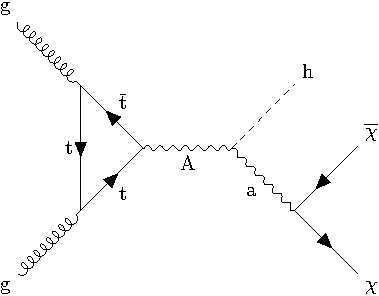
\includegraphics[width=0.4\textwidth]{figures/Feyn-2HDMa.pdf}}\hspace{1cm}
 \subfloat{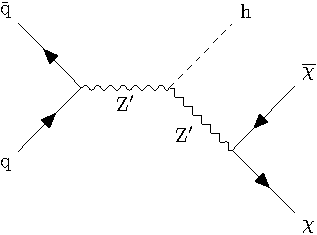
\includegraphics[width=0.34\textwidth]{figures/Feyn-Baryonic.pdf}} \\
\caption{Feynman diagrams for the 2HDM+a model (left) and the Baryonic Z' model (right).}
\label{feyns}
\end{figure}


%The quantity \ptvecmiss, calculated as the negative vectorial sum of the transverse momentum (\pt) of all objects identified in an event, 
%represents the total
%momentum carried by the DM particles.
%The magnitude of this vector is referred to as \MET.
%For a given value of \mzp, the \pt of the \Az decreases as its mass increases.
%Therefore, the \MET spectrum softens with increasing \Az masses.
%A comparison of the \MET distributions expected from representative scenarios of the \cPZpr-2HDM model and the \cPZpr-Baryonic model are presented in Fig.~\ref{fig:met_signals}.


%\begin{figure}
%\centering
%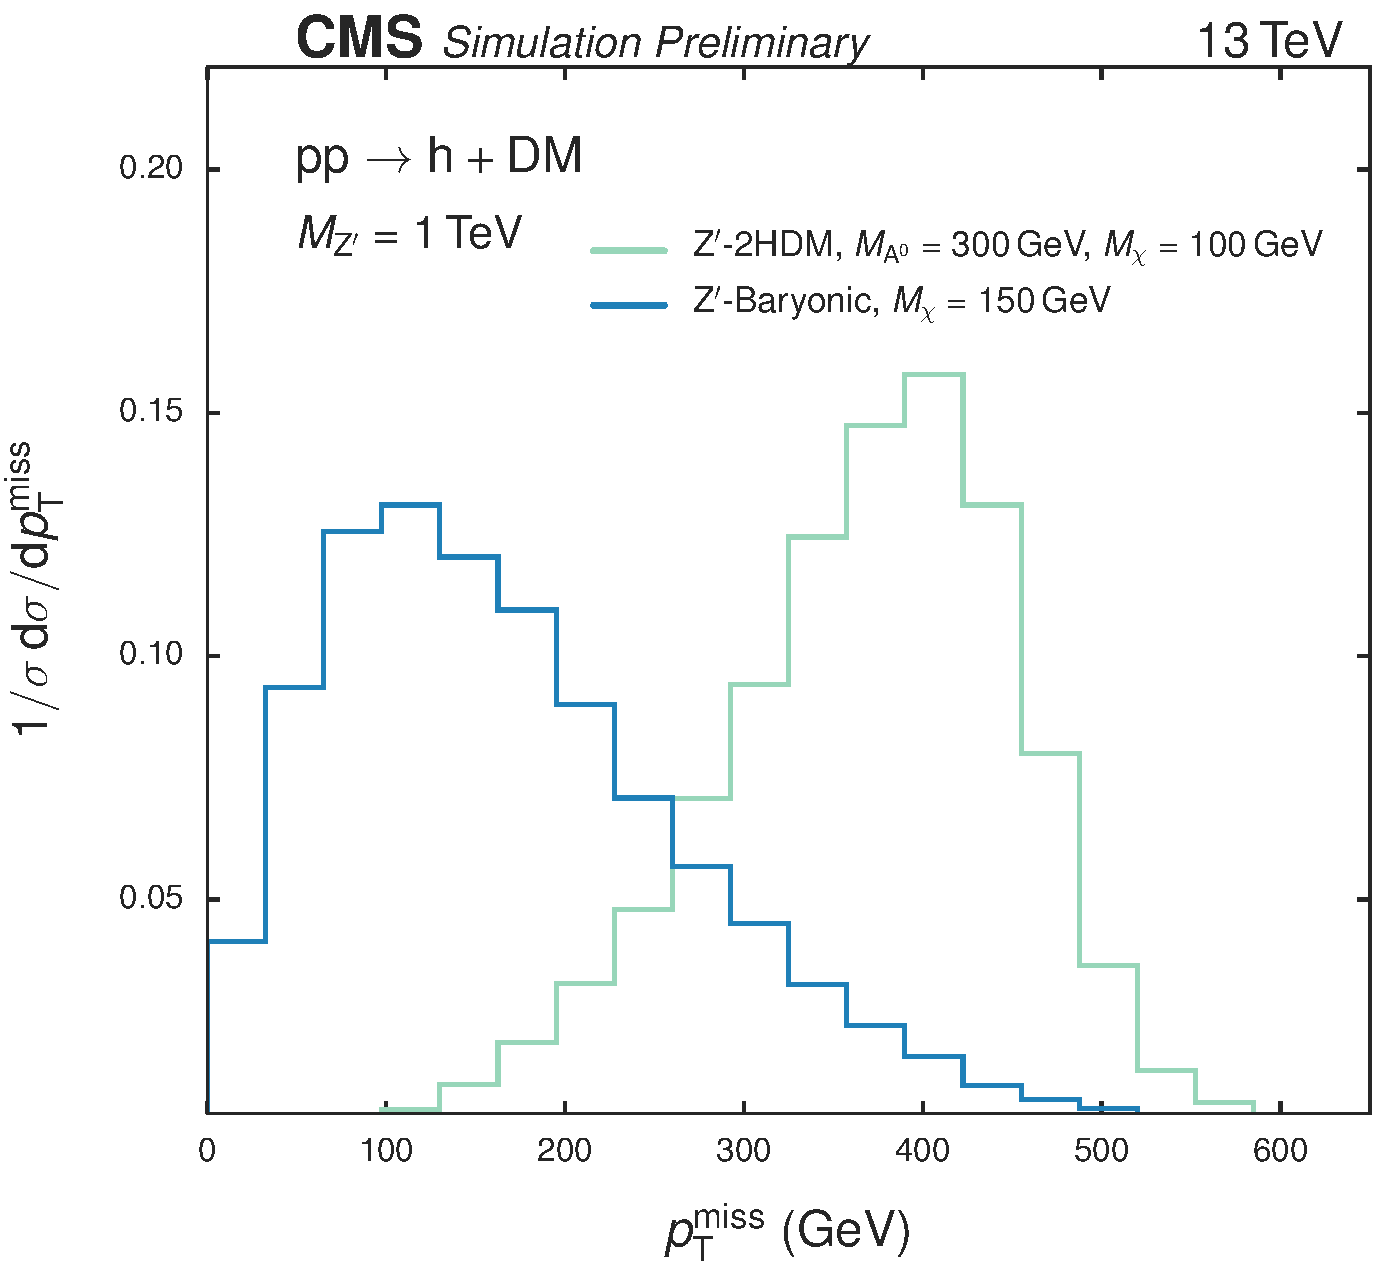
\includegraphics[width=0.55\textwidth]{figures/puppimet_signals.pdf}
%\includegraphics[width=0.45\textwidth]{figures/ZpBaryonicModel.pdf}
%\caption{Reconstructed \MET for representative scenarios of two $\mathrm{h}+\mathrm{DM}$ models investigated. Coupling parameters are chosen as mentioned in the text. The \cPZpr-2HDM model in general has a significant harder \MET~spectrum than the \cPZpr-Baryonic model, which makes the former easier to distinguish from SM background processes.}
%\label{fig:met_signals}
%\end{figure}

Signal events are characterized by a large imbalance in the transverse momentum(or hadronic recoil), that indicates the presence of invisible DM particles, and by hadronic activity consistent with the production of a SM Higgs boson that decays into a b quark pair. Requirements on the mass of the reconstructed Higgs boson candidate, together with the identification of the products of hadronization of the two b quarks produced in the Higgs boson decay, define a data sample that is expected to be enriched in signal events. Several different SM processes can mimic such topology, like top quark pair production and the production of a vector boson (V) in association with multiple jets. Data in statistically independent control samples are used to predict the hadronic recoil distribution for these SM processes that constitute the largest source of background.
Both signal and background contributions to the data are extracted with a likelihood fit to the hadronic recoil distribution, performed simultaneously in all the different analysis subsamples.
